\chapter{Implementazione e Verifica}

\section{Componenti grafici}

\section{Gestione dello stato}
Il framework \textit{KVision}, oltre a fornire strumenti e metodi di programmazione molto robusti e versatili, dona la possibilità di usare tutta la capacità della libreria di \textit{Redux}\footnote{\url{https://redux.js.org/tutorials/essentials/part-1-overview-concepts}}, una libreria open-source per la gestione dello stato delle applicazioni JavaScript. Il fulcro di questa libreria consiste nel cosiddetto \textit{store}, un archivio centralizzato per uno stato che deve essere condiviso in tutta l'applicazione, attraverso l'utilizzo di regole che garantiscono che lo stato possa essere aggiornato solamente in modo prevedibile. Analizziamo ora il funzionamento della gestione dello stato introducendo tutti i concetti chiave: 
\begin{itemize}	
	\item \textbf{State}: ``The source of truth that drives our app'', in altre parole, dati o insieme di dati che influenzano il comportamento o l'aspetto dell'applicazione. 	
	\item \textbf{View}: una descrizione dichiarativa dell'interfaccia utente basata sullo stato attuale.
	\item \textbf{Actions}: usati per descrivere possibili cambiamenti dello stato. Sono oggetti, dotati di un campo che ne indica il tipo, incaricati a indicare l'azione che deve essere eseguita sullo store per cambiarne lo stato. Si può pensare a questo tipo di oggetti come ad eventi che riportano un certo avvenimento nell'applicazione. Di solito vengono chiamati dopo un input, ovvero quando si verifica un evento specifico nell'applicazione, come un click del mouse o quando un pulsante viene premuto.
	\item \textbf{Store (archivio)}: l'oggetto centrale che contiene lo stato dell'applicazione in un determinato momento.
	\item \textbf{Reducers}: funzioni che descrivono esattamente come deve essere cambiato lo stato, in risposta alle azioni chiamate sullo store. Come parametri di ingresso accettano lo stato corrente e l'azione che si vuole eseguire, ritornando un nuovo stato. I reducer possono essere paragonati a dei \textit{listener} che gestiscono gli eventi (\textit{actions}) in base al loro tipo.
	\item \textbf{Dispatch}: metodo di cui lo store dispone. L'unico modo per aggiornare lo stato è invocando questa funzione, passando come parametro un'azione.  A questo punto lo store può eseguire il suo \textit{reducer} e salvare il nuovo stato al suo interno. Nel momento in cui un evento viene innescato (proveniente per esempio della UI), si vuole di conseguenza aggiornare il valore dello store.
	\item \textbf{Subscribe}: sono funzioni che permettono ai componenti grafici di ``iscriversi'' ai cambiamenti di stato dello store. Ogni volte che lo stato cambia, i componenti iscritti vengono avvisati, dando la possibilità di aggiornare la UI in base al nuovo cambio di stato.
\end{itemize}
Insieme agli elementi appena descritti, la figura \cref{fig:redux-scheme} riesce a dare una visione più completa.
\begin{figure}[htb]
	\centering
	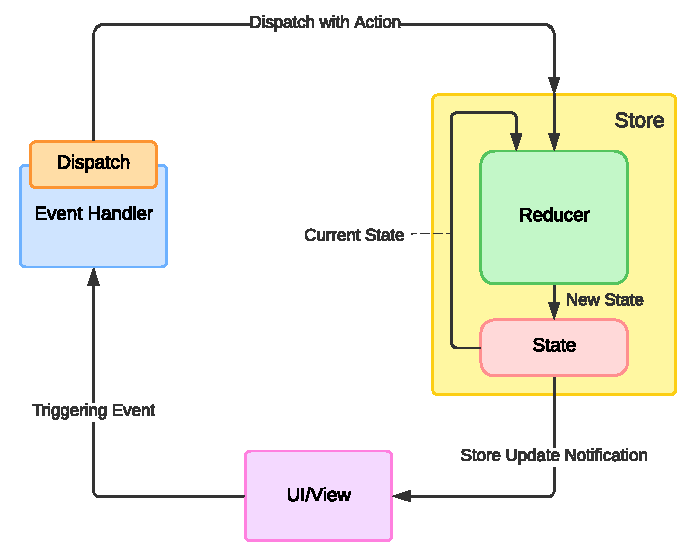
\includegraphics[scale=0.8]{imgs/Redux_Scheme.pdf}
	\caption{Architettura generale del client web}
	\label{fig:redux-scheme}
\end{figure}
Dallo schema è possibile notare come sia presente una unica direzione che collega le varie entità. Questo è dovuto al fatto che la sequenza dei passi da compiere per l'aggiornamento dello stato segue il paradigma ``one-way data flow". In particolare, per Redux si seguono quindi questi passaggi:
%Viene creato uno store Redux utilizzando una funzione reducer radice.
%Lo store chiama il reducer radice una volta e salva il valore restituito come suo stato iniziale.
%Quando l'interfaccia utente viene renderizzata per la prima volta, i componenti dell'interfaccia utente accedono allo stato attuale dello store Redux e utilizzano tali dati per decidere cosa renderizzare. Si iscrivono anche a eventuali aggiornamenti futuri dello store in modo da poter sapere se lo stato è cambiato.

\begin{enumerate}	
	\item Qualcosa accade nell'applicazione, come un utente che fa clic su un pulsante.
	\item Viene chiamata la funzione \texttt{dispatch}, specificando l'azione per modificare lo store Redux.
	\item Lo store esegue la funzione reducer con lo stato precedente e l'azione corrente, e salva il valore restituito come nuovo stato.
	\item Lo store notifica a tutte le parti dell'interfaccia utente che sono iscritte che lo store è stato aggiornato.
	\item Ciascun componente dell'interfaccia utente che necessita dei dati dallo store controlla se le parti dello stato di cui hanno bisogno sono cambiate.
	\item Ciascun componente che rileva che i suoi dati sono cambiati forza un nuovo rendering con i nuovi dati, così da poter aggiornare ciò che viene mostrato sullo schermo.
\end{enumerate}
Per mantenere l'informazione ottenuto dalla query sullo stato di un nodo lo store che ne deriva viene dichiarato come in \cref{lst:redux-node-store}.
\lstinputlisting[language=Kotlin,label={lst:redux-node-store}]{listings/Store.kt}.

\texttt{createTypedReduxStore} è una funzione della libreria di \textit{KVision} che permette la creazione

\section{Integrazioni di operazioni GraphQL}

\section{Verifica}